\chapter{Principios físicos}

El objetivo de esta clase es familiarizarze con los conceptos de combinación de bandas y firma espectral \emph{SNAP (Sentinel Aplication Toolbox)}. Se realizará diferentes combinaciones de bandas teniendo en cuenta la respuesta de los usos y coberturas en función de la combinación de colores. Respuesta espectral de usos y coberturas.





\section{Combinación de bandas}
En esta ocasión vamos a realizar diferentes combinaciones de bandas analizando la variación en la visualización de los diferentes usos y coberturas. 

%desarrollar un poco

\section{Combinación color real}

Abra la imagen \begin{center} \directory{S2B\_MSIL2A\_2018-01-31.dim}.
\end{center} seleccione \menu{Open RGB image windows} haciendo click derecho sobre el nombre de la imagen. Se desplegará una nueva ventana (Figura \ref{fig:RGB}) que le permitirá elegir la combinación de bandas. Por defecto aparecerá la combinación color real que utiliza las bandas \emph{rojo (4)}, \emph{verde(3)} y \emph{azul(2)} de \emph{Sentinel-2}. Desplieguela haciendo click en OK. En esta combinación las características del suelo aparecen en colores similares a su apariencia para el sistema visual humano, la vegetación sana se observa en tonalidades de verde, suelos recientemente cosechados o compactados se observan brillantes, en tanto que la vegetación senescente o de escasa cobertura se observa en tonos de marrón y amarillo. Por otro lado, esta combinación de bandas presenta mayor respuesta a cuerpos de agua, resaltando características como sedimentos, profundidad o presencia de floraciones algales. 

Utilice el mapa con puntos de interés para identificar y familiarizarse con los diferentes usos y coberturas (Figura \ref{fig:mapa}). Explore la ubicación de los puntos mencionados utilizando las herramientas de navegación y zoom  (Figura \ref{fig:mono}). Compare color, tono y textura para cada punto. 


\section{Combinación infrarrojo color}

Seleccione \menu{Open RGB image windows} haciendo click derecho sobre el nombre de la imagen. Se desplegará una nueva ventana (Figura \ref{fig:RGB}) que le permitirá elegir la combinación de bandas. Seleccione las bandas \emph{infrarrojo cercano (8)}, \emph{verde(3)} y \emph{azul(2)} de \emph{Sentinel-2}. Desplieguela haciendo click en OK. En esta combinación las características del suelo aparecen en colores similares a su apariencia para el sistema visual humano, la vegetación sana se observa en tonalidades de verde, suelos recientemente cosechados o compactados se observan brillantes, en tanto que la vegetación senescente o de escasa cobertura se observa en tonos de marrón y amarillo. Por otro lado, esta combinación de bandas presenta mayor respuesta a cuerpos de agua, resaltando características como sedimentos, profundidad o presencia de floraciones algales. 

Utilice el mapa con puntos de interés para identificar y familiarizarse con los diferentes usos y coberturas (Figura \ref{fig:mapa}). Explore la ubicación de los puntos mencionados utilizando las herramientas de navegación y zoom  (Figura \ref{fig:mono}). Compare color, tono y textura para cada punto. 

\section{Consulta de píxel}

Para obtener información sobre un pixel seleccione la pestaña \menu{Pixel info}, junto al \menu{Product explorer} (Figura \ref{fig:pixel}), y posicionese  sobre uno en la imagen.

\begin{figure}[h!]
    \centering
    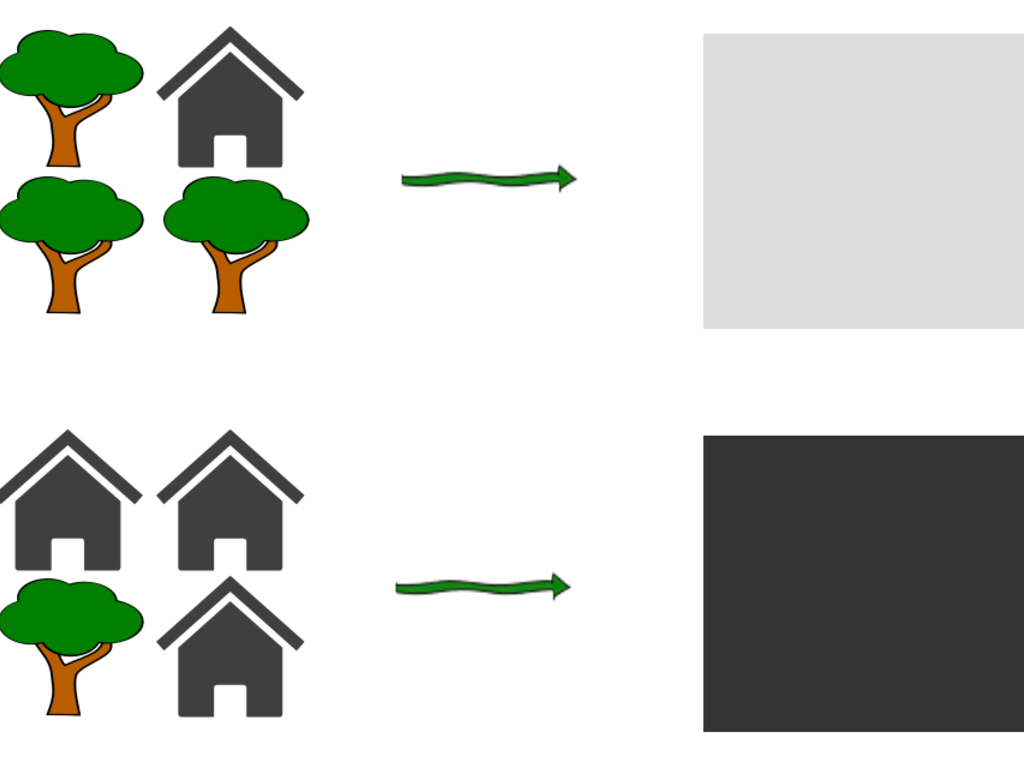
\includegraphics[width=0.3\textwidth]{fig:pixel.png}
    \caption{Herramienta de consulta de píxel. Puede verse la posición del píxel en la imagen, su latitud y longitud y el valor del píxel para la banda desplegada.}
    \label{fig:pixel}
\end{figure}

Allí encontrará la latitud y longitud, las coordenadas dentro del mapa y el valor del pixel en la banda abierta.

\section{Multiples visualizadores}

Abra las imágenes
\begin{center} \directory{S2B\_MSIL2A\_2018-01-31.dim}.
\end{center}
y
\begin{center} \directory{MCD43A4.A2018039.h13v11.0065.dim}.
\end{center}

y desplieguelas en combinación de color RGB. Las tres corresponden a la misma zona durante el mes de enero de 2018.

Para ver las tres en simultaneo haga click en \menu{Window>Tile Horizontally} mostrandose de esa manera las imágenes vinculadas una junto a la otra. Moverse o hacer zoom en una imagen lo reproducirá en las otras. Para volver al modo habitual haga click en \menu{Window>Tile Single}.

\section{Actividad práctica}

\begin{enumerate}
  \item Identifique en la imagen los siguientes objetos:
  \begin{enumerate}
    \item El río Iguazú que recorre la imagen de izquierda a derecha en color gris/marron.
    \item El río Paraná que corta la imagen de arriba a abajo celestre.
    \item La ciudad de Puerto Iguazú al sur-este del cruce de los rios Iguazú y Paraná.
    \item La zonas cultivadas al norte del río Iguazú con formas de parches en color verde.
    \item Laz onas cultivadas al oeste del río Paraná formadas por parches de color verde, con cultivo, y rosa, sin cultivo.
    \item La selva Paranaense al sur del río Iguazú en color verde.
    \item El embalse Urugua-í al sur de la imagen.
    \item La zona de forestaciones en color verde más oscuro entre la selva Paranaense y el embalse Urugua-í.
    \item El aeropuerto de cataratas del Iguazú en medio de la selva Paranaense.
  \end{enumerate}

  \item Mida dentro de las tres imágenes los siguientes objetos:
  \begin{enumerate}
    \item El largo de la pista de aterrizaje del aeropuerto.
    \item El ancho del río Paraná frente a la ciudad de Puerto Iguazú.
    \item El perímetro de la ciudad de puerto Iguazú.
    \item El perímetro del parche de selva Paranaense al norte del río Iguazú.
    \item El tamaño de un píxel.
  \end{enumerate}

  \item Identifique las coordenadas geográficas de los siguientes objetos:
  \begin{enumerate}
    \item El aeropuerto de las cataratas del Iguazú.
    \item La ciudad de Puerto Iguazú.
    \item La ciudad de Foz de Iguazú.
    \item Ciudad del este.
    \item La desembocadura del embalse Urugua-Í.
    \item El cruce entre los ríos Paraná y Iguazú.
    \item Las cataratas del Iguazú donde el río Iguazú se angosta.
  \end{enumerate}

\end{enumerate}
